\documentclass[conference,10pt,letterpaper]{IEEEtran}
\usepackage[T1]{fontenc}
\usepackage{amsmath,amssymb,bm,booktabs,cite}
\usepackage{graphicx,tikz,pgfplots}
\usepackage[hidelinks]{hyperref}
\usetikzlibrary{arrows.meta,positioning,calc}
\usepgfplotslibrary{statistics,groupplots}
\pgfplotsset{compat=1.18}
\definecolor{valColor}{RGB}{38,118,168}
\definecolor{testColor}{RGB}{216,121,39}
\definecolor{emptycolor}{RGB}{75,75,75}
\definecolor{occColor}{RGB}{181,41,54}
\newcommand{\SelectedFeatures}{CSI}
\newcommand{\SelectedModel}{LR}
\newcommand{\ValBA}{84.4}
\newcommand{\TestBA}{66.1}
\newcommand{\TestAUC}{0.708}
\newcommand{\ValAUC}{0.901}
\newcommand{\SelectedThreshold}{0.4707}
\newcommand{\FitDots}{51,287}
\newcommand{\TestTN}{59}
\newcommand{\TestFP}{37}
\newcommand{\TestFN}{28}
\newcommand{\TestTP}{68}
\newcommand{\ValPackets}{1,113,472}
\newcommand{\ValFrames}{106,150}
\newcommand{\ValSelectedPackets}{922,551}
\newcommand{\ValSelectedFrames}{88,500}
\newcommand{\ValInterpolation}{7.9}
\newcommand{\ValValidSeconds}{45}
\newcommand{\ValPacketRate}{101.1}
\newcommand{\TestPackets}{1,217,863}
\newcommand{\TestFrames}{90,432}
\newcommand{\TestSelectedPackets}{922,641}
\newcommand{\TestSelectedFrames}{65,312}
\newcommand{\TestInterpolation}{12.6}
\newcommand{\TestValidSeconds}{39}
\newcommand{\TestPacketRate}{83.8}
\newcommand{\CsiBA}{66.1}
\newcommand{\SnrFusionBA}{65.6}
\newcommand{\RdBA}{65.1}
\newcommand{\RdAUC}{0.760}
\newcommand{\RaBA}{68.2}
\newcommand{\AllBA}{66.1}
\newcommand{\ResultRows}{%
CSI & LR & 0.844 & 0.661 & 0.708 \\
CSI+SNR+RE & RF & 0.838 & 0.672 & 0.753 \\
CSI+SNR & LR & 0.838 & 0.656 & 0.723 \\
CSI+SNR+XY & RF & 0.837 & 0.667 & 0.739 \\
CSI+SNR+RA & RF & 0.831 & 0.682 & 0.739 \\
CSI+SNR+RD & RF & 0.831 & 0.651 & 0.760 \\
CSI+radar all & RF & 0.825 & 0.661 & 0.696 \\
RD & LR & 0.681 & 0.490 & 0.274 \\
SNR & LR & 0.637 & 0.641 & 0.662 \\
Radar all & RF & 0.613 & 0.620 & 0.771 \\
XY & LR & 0.600 & 0.365 & 0.217 \\
RA & LR & 0.600 & 0.349 & 0.228 \\
RE & LR & 0.500 & 0.510 & 0.516 \\
}

\newcommand{\E}{\mathbb{E}}
\newcommand{\R}{\mathbb{R}}
\newcommand{\C}{\mathbb{C}}
\DeclareMathOperator{\med}{median}
\DeclareMathOperator{\Var}{Var}
\DeclareMathOperator{\mean}{mean}
\title{Multimodal Wireless Sensing for Room Occupancy:\\Uniform-Rate CSI Variance and FMCW Radar}
\author{\IEEEauthorblockN{Gad Gad\IEEEauthorrefmark{1}, Iqra Batool\IEEEauthorrefmark{1}, Mostafa Fouda\IEEEauthorrefmark{2},\\Shikhar Verma\IEEEauthorrefmark{3}, Zubair Md Fadlullah\IEEEauthorrefmark{1}}
\IEEEauthorblockA{\IEEEauthorrefmark{1}Department of Computer Science, Western University, London, ON, Canada\\
\IEEEauthorrefmark{2}Department of Electrical and Computer Engineering, Idaho State University, Pocatello, ID, USA\\
\IEEEauthorrefmark{3}School of Informatics, Kochi University of Technology, Kochi, Japan}}
\begin{document}
\maketitle
\begin{abstract}
Room occupancy sensing must detect both moving and stationary occupants despite intermittent measurements and changing propagation conditions. We study lightweight fusion of WiFi channel state information (CSI) and frequency-modulated continuous-wave radar using 1,523 labeled minute recordings. CSI amplitudes are resampled to a uniform 100 Hz grid before fixed two-dimensional principal component analysis. A three-second projection-variance statistic is combined with radar signal-to-background and range--Doppler, range--azimuth, range--elevation, and XY energy descriptors. Both evaluation sets are class-balanced: validation contains 80 empty and 80 occupied minutes, and test contains 96 of each. We define the two signal branches mathematically from observations to classification and evaluate 26 conventional model/input combinations. The validation-selected \SelectedFeatures{} (\SelectedModel{}) achieves \TestBA\% test balanced accuracy and \TestAUC{} ROC AUC. Native-rate and interpolated-sample coverage are audited separately. Results remain exploratory because these sessions have been inspected during development; uniform sampling and multimodal fusion do not by themselves establish improved generalization.
\end{abstract}
\begin{IEEEkeywords}
Room occupancy, WiFi CSI, FMCW radar, sensor fusion, principal component analysis, resampling.
\end{IEEEkeywords}

\section{Introduction}
Room occupancy differs from motion detection: an occupied room may contain a seated, standing, or sleeping person with little movement. Radar evidence can be weak outside its field of view, while CSI reflects multipath changes along wireless propagation paths. Their complementary sensitivities motivate fusion, but noise, gaps, and acquisition changes can also produce correlated errors. Our objective is binary occupancy in the room containing the collection devices.

The supplied WiFi-sensing manuscript~\cite{wifi} motivates amplitude-based processing with inexpensive receivers. We combine its channel model with the FMCW signal formulation in HOOD~\cite{hood}, then define the specific processing used in this collection. The contribution is an auditable end-to-end baseline, not a claim that radar--WiFi fusion or efficient classification is new. A uniform input rate, fixed feature coordinates, chronological partitions, and explicit coverage accounting make the empirical comparison reproducible.

Our CSI feature measures the dispersion of three consecutive one-second PCA observations. It is not the cumulative distance traveled by the projections. Radar contributes a signal-to-background proxy and compact map summaries. We compare logistic regression (LR) and random forests (RF) with identical evaluation minute IDs. The study reports availability and classification together and separates processed 100 Hz sampling from the actual rate at which packets arrive.

\section{Related Work}
DeMan addresses moving and stationary presence using WiFi measurements, including breathing-related evidence~\cite{deman}. SHARP studies activity recognition with Doppler information derived from phase-processed CSI~\cite{sharp}. LiteHAR investigates efficient random-convolution features and ridge classification~\cite{litehar}. These methods motivate sensitivity to subtle motion and processing cost, but their datasets and tasks do not provide directly comparable numerical baselines here.

HOOD uses macro/micro range--Doppler images and reconstruction-based learning for human presence and out-of-distribution detection~\cite{hood}. We use its FMCW physical formulation as a starting point, while implementing conventional FFT and beamforming descriptors. HOOD's micro-RDI stacking, E-RESPD, and neural architecture are not components of this experiment. Radar--WiFi learned fusion has also been studied~\cite{fusion}; our focus is interpretable features and temporal transfer within a measured collection.

\begin{figure*}[t]
\centering\resizebox{\textwidth}{!}{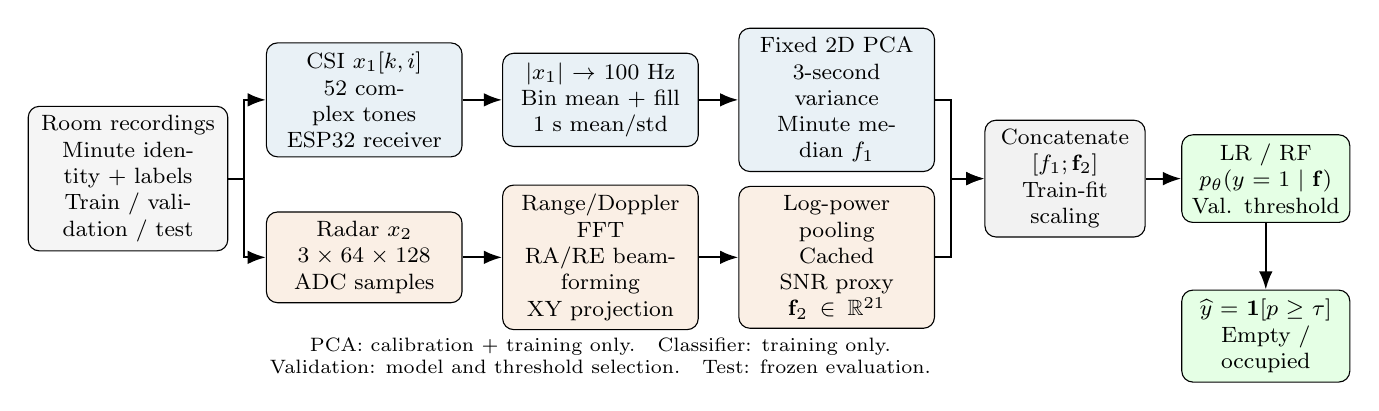
\begin{tikzpicture}[>=Latex,font=\footnotesize,
 source/.style={draw,rounded corners,fill=gray!8,align=center,text width=2.3cm,minimum height=1.05cm},
 process/.style={draw,rounded corners,align=center,text width=2.25cm,minimum height=1.05cm},
 arrow/.style={->,thick},every edge/.style={arrow}]
\node[source] (data) at (0,0) {Room recordings\\Minute identity + labels\\Train / validation / test};
\node[process,fill=valColor!10] (wifi) at (3,1) {CSI $x_1[k,i]$\\52 complex tones\\ESP32 receiver};
\node[process,fill=valColor!10] (csi) at (6,1) {$|x_1|\to100$ Hz\\Bin mean + fill\\1 s mean/std};
\node[process,fill=valColor!10] (pca) at (9,1) {Fixed 2D PCA\\3-second variance\\Minute median $f_1$};
\node[process,fill=testColor!12] (radar) at (3,-1) {Radar $x_2$\\$3\times64\times128$\\ADC samples};
\node[process,fill=testColor!12] (maps) at (6,-1) {Range/Doppler FFT\\RA/RE beamforming\\XY projection};
\node[process,fill=testColor!12] (pool) at (9,-1) {Log-power pooling\\Cached SNR proxy\\$\mathbf f_2\in\mathbb R^{21}$};
\node[process,fill=gray!10,text width=1.8cm] (fusion) at (11.9,0) {Concatenate\\$[f_1;\mathbf f_2]$\\Train-fit scaling};
\node[process,fill=green!10,text width=1.9cm] (learn) at (14.45,0) {LR / RF\\$p_\theta(y=1\mid\mathbf f)$\\Val. threshold};
\node[process,fill=green!10,text width=1.9cm] (output) at (14.45,-2) {$\widehat y=\mathbf{1}[p\geq\tau]$\\Empty / occupied};
\draw[arrow] (data.east) -- ++(.2,0) |- (wifi.west);
\draw[arrow] (data.east) -- ++(.2,0) |- (radar.west);
\draw[arrow] (wifi) -- (csi);\draw[arrow] (csi) -- (pca);
\draw[arrow] (radar) -- (maps);\draw[arrow] (maps) -- (pool);
\draw[arrow] (pca.east) -- ++(.2,0) |- (fusion.west);
\draw[arrow] (pool.east) -- ++(.2,0) |- (fusion.west);
\draw[arrow] (fusion) -- (learn);\draw[arrow] (learn) -- (output);
\node[align=center,font=\scriptsize] at (6,-2.25) {PCA: calibration + training only.\quad Classifier: training only.\\Validation: model and threshold selection.\quad Test: frozen evaluation.};
\end{tikzpicture}
}
\caption{Data sources, processing branches, and learning protocol. The input symbols $x_1$ and $x_2$ are defined in Section~\ref{sec:model}. CSI is resampled before summary extraction and PCA. Fusion operates on minute-level features, not hardware-synchronized samples.}
\label{fig:overview}
\end{figure*}

\section{System Model}\label{sec:model}
Let $m$ index a nominal minute, $i$ a CSI packet, and $k$ a retained subcarrier. Radar indices are frame $f$, receiver $r$, chirp $c$, and fast-time sample $n$. The observed modalities are $x_1$ (complex CSI) and $x_2$ (real radar ADC data). The label is $y_m=0$ for empty and $y_m=1$ for occupied; sleep is mapped to occupied during training.

\subsection{WiFi observation $x_1$}
Following the supplied channel model~\cite{wifi}, define
\begin{align}
x_1[k,i]&=H_k(t_i)e^{j\phi_k(t_i)}+\eta_1[k,i],\label{eq:wifi}\\
H_k(t)&=\sum_{\ell=1}^{L}a_\ell(t)e^{-j2\pi(f_{\rm W}+k\Delta f)\tau_\ell(t)}.\label{eq:paths}
\end{align}
Here $a_\ell$ and $\tau_\ell$ are path gain and delay; $\eta_1$ is observation noise. Hardware phase terms can be represented as
\begin{equation}
\phi_k=-2\pi k(\tau_{\rm SFO}+\tau_{\rm PDD})/T
+\phi_{\rm CFO}+\phi_{\rm PPO}+\phi_{\rm PA}.
\end{equation}
The experiment retains 52 subcarriers and uses $A_k(t_i)=|x_1[k,i]|$. No phase sanitization is applied. This removes an ideal multiplicative phase factor but does not remove gain drift or measurement noise. Motion and stationary occupancy can perturb the paths differently; amplitude variation is not a calibrated displacement.

\subsection{FMCW observation $x_2$}
Using the chirp model in~\cite{hood}, with slope $S=B/T_c$,
\begin{equation}
s(t)=\exp\{j2\pi(f_{\rm R}t+St^2/2)\},\quad 0\leq t<T_c.
\end{equation}
A useful narrowband, constant-velocity approximation to the mixed and digitized return is
\begin{align}
x_2^{(f)}[r,c,n]&=\Re\Big\{\sum_{\ell}\beta_{\ell,f}
 e^{j\psi_{\ell,r,c,n}}\Big\}+\eta_2^{(f)}[r,c,n],\\
\psi_{\ell,r,c,n}&=2\pi\Big(f_{b,\ell}\frac{n}{f_{\rm ADC}}
+f_{D,\ell}cT_{\rm rep}+\frac{\mathbf d_r^T\mathbf u_\ell}{\lambda}\Big)
+\varphi_\ell.\label{eq:radar}
\end{align}
The approximate beat and Doppler frequencies are $f_b\simeq2SR/c_0$ and $f_D=2v/\lambda$, subject to mixer convention and range--Doppler coupling. The receiver displacement is $\mathbf d_r$ and target direction is $\mathbf u_\ell$. Our decoded frame has $N_R=3$, $N_c=64$, and $N_s=128$, with packed 12-bit ADC samples. These dimensions are observed in the collection. HOOD's RF settings are not assumed to be this dataset's settings: physical range, velocity, and angle calibration have not been verified.

\section{Data Collection and Evaluation Sets}\label{sec:data}
\subsection{Collection organization}
The 1,523 labeled minute folders comprise 808 calibration, 274 training, 192 validation, and 249 test recordings. Manifests identify ESP32 CSI and DreamHAT radar, stored as chunked files or synchronized-capture containers. One CSI receiver stream is selected by packet coverage. Recording identity and host timing pair the modalities; hardware-trigger synchronization is not established. Room dimensions, participant count, and exact sensor positions remain unverified in available metadata. The target is presence in the collection room, including sitting, standing, and walking; these postures are not separate test labels.

\begin{table}[t]
\centering\caption{Collection and evaluation counts in nominal minutes. E/S/P: empty/sleep/present. Sleep is occupied for binary training.}
\label{tab:data}\footnotesize
\begin{tabular}{lccc}\toprule
Partition & Dates, 2026 & Collected E/S/P & Evaluated E/S/P\\\midrule
Calibration & Aug. 17--18 & 0/808/0 & PCA only\\
Training & Sep. 6--8 & 188/16/70 & 184/16/68\\
Validation & Sep. 15 & 112/0/80 & 80/0/80\\
Test & Sep. 16--17 & 96/0/153 & 96/0/96\\\bottomrule
\end{tabular}
\end{table}

\subsection{Validation dataset}
Validation was collected on 15 September, from 19:41 to 23:08 by local folder timestamps, with gaps. It contains 112 empty and 80 present minute recordings, without sleep labels. The selected stream supplies \ValPackets{} decoded CSI packets; map extraction uses \ValFrames{} radar frames. All required features are available for all 192 minutes. A fixed balanced subset contains 80 empty and all 80 present minutes, with \ValSelectedPackets{} CSI packets and \ValSelectedFrames{} radar frames over 160 nominal minutes. This later acquisition session selects models and thresholds, but does not fit PCA or scaling.

\subsection{Test dataset}
Test was collected overnight from 22:10 on 16 September to 02:45 on 17 September. It contains 96 empty and 153 present minutes; no sleep class is available. There are \TestPackets{} decoded CSI packets and \TestFrames{} radar frames in the original collection. The balanced subset contains all 96 empty and 96 sampled present minutes, with \TestSelectedPackets{} packets and \TestSelectedFrames{} frames. Test labels follow the acquisition schedule, with empty beginning at 01:10; they are not independently frame-verified. Acquisition identifiers differ ($t$ versus $pi$), but these identifiers alone do not establish a change of room or geometry.

\subsection{Balance and coverage}
Majority-class undersampling within each evaluation partition uses chronologically sorted minute IDs and seed 42, without replacement. The selected 160 validation and 192 test minutes are identical to the preceding experiment. The discarded 32 validation-empty and 57 test-present minutes remain in the collection audit. They are not sensor failures. No overlapping window is assigned across partitions.

The training cohort contains 184 empty and 84 occupied minutes after six radar/SNR exclusions. Calibration supplies PCA observations only. The reported baseline uses class-weighted learning on these 268 unique training minutes. Class weighting equalizes the classes' contributions to the training objective; it does not change the number of unique recordings or generate synthetic observations.

\begin{figure}[t]
\centering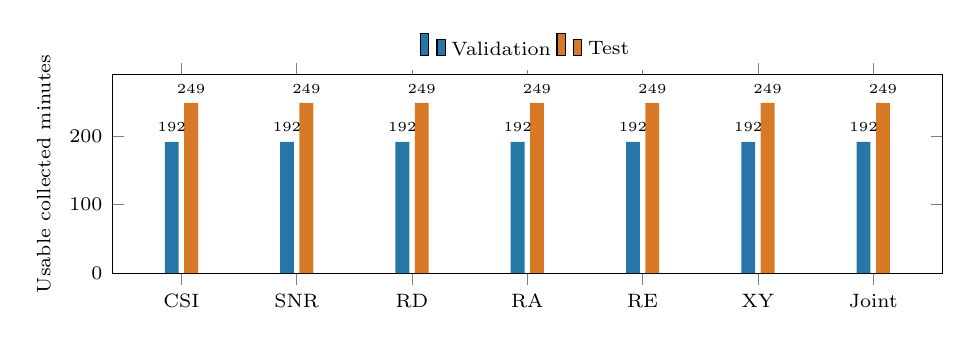
\begin{tikzpicture}
\begin{axis}[width=\columnwidth,height=4.1cm,ybar,bar width=5pt,ymin=0,ymax=290,symbolic x coords={CSI,SNR,RD,RA,RE,XY,Joint},xtick=data,tick label style={font=\scriptsize},ylabel={Usable collected minutes},label style={font=\scriptsize},legend style={at={(.5,1.02)},anchor=south,font=\scriptsize,legend columns=2,draw=none},nodes near coords,nodes near coords style={font=\tiny},enlarge x limits=.1]
\addplot[fill=valColor,draw=none] coordinates {(CSI,192) (SNR,192) (RD,192) (RA,192) (RE,192) (XY,192) (Joint,192)};
\addplot[fill=testColor,draw=none] coordinates {(CSI,249) (SNR,249) (RD,249) (RA,249) (RE,249) (XY,249) (Joint,249)};
\legend{Validation,Test}
\end{axis}
\end{tikzpicture}
\caption{Feature availability before class balancing. CSI and radar are the two physical modalities; SNR, RD, RA, RE, and XY share the radar source. All collected evaluation minutes have the required features.}
\label{fig:coverage}
\end{figure}

\section{Processing and Fusion}\label{sec:processing}
\subsection{Guaranteed 100 Hz CSI grid}
Within each minute, finite CSI observations are restricted to $[0,60)$ seconds, sorted, and deduplicated. The guaranteed-rate method from the companion WiFiSensing code is executed unchanged with $F=100$ Hz. Let $t_0$ be the first observed timestamp and $u_j=t_0+j/F$. Centered bins define
\begin{align}
\mathcal I_j&=\{i:u_j-1/(2F)\leq t_i<u_j+1/(2F)\},\\
\widetilde A_k[j]&=\frac{1}{|\mathcal I_j|}\sum_{i\in\mathcal I_j}A_k(t_i),
\quad |\mathcal I_j|>0.\label{eq:resample}
\end{align}
There are $J=\lceil F(t_{\rm last}-t_0)\rceil$ bins; endpoint assignments are clipped into the first/last bin as in the source routine. Empty bins between populated $j_-$ and $j_+$ are interpolated:
\begin{equation}
\widetilde A_k[j]=(1-\alpha_j)\widetilde A_k[j_-]+\alpha_j\widetilde A_k[j_+],\quad
\alpha_j=\frac{u_j-u_{j_-}}{u_{j_+}-u_{j_-}}.\label{eq:interpolation}
\end{equation}
Thus 100 Hz is a processed-grid rate, not a guarantee of received packets. Median native packet rates are \ValPacketRate{} and \TestPacketRate{} Hz for validation and test. Among samples used in accepted summaries, median interpolated fractions are \ValInterpolation\% and \TestInterpolation\%, respectively (Fig.~\ref{fig:temporal}).

\begin{figure}[t]
\centering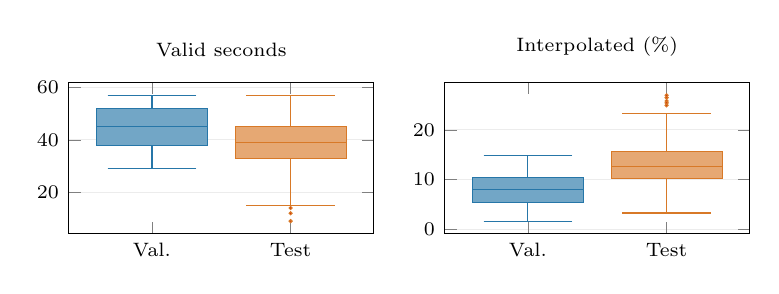
\begin{tikzpicture}
\begin{groupplot}[group style={group size=2 by 1,horizontal sep=.9cm},width=.45\columnwidth,height=3.5cm,boxplot/draw direction=y,xtick={1,2},xticklabels={Val.,Test},xmin=.4,xmax=2.6,tick label style={font=\scriptsize},title style={font=\scriptsize},ymajorgrids,grid style={gray!15}]
\nextgroupplot[title={Valid seconds}]
\addplot+[boxplot prepared={lower whisker=29,lower quartile=38,median=45,upper quartile=52,upper whisker=57},boxplot/draw position=1,fill=valColor!65,draw=valColor,mark=*,mark size=.55pt] coordinates {};
\addplot+[boxplot prepared={lower whisker=15,lower quartile=33,median=39,upper quartile=45,upper whisker=57},boxplot/draw position=2,fill=testColor!65,draw=testColor,mark=*,mark size=.55pt] coordinates {(2,9) (2,14) (2,12)};
\nextgroupplot[title={Interpolated (\%)}]
\addplot+[boxplot prepared={lower whisker=1.60377358,lower quartile=5.28888045,median=7.89529725,upper quartile=10.4327493,upper whisker=14.8888889},boxplot/draw position=1,fill=valColor!65,draw=valColor,mark=*,mark size=.55pt] coordinates {};
\addplot+[boxplot prepared={lower whisker=3.23636364,lower quartile=10.1521739,median=12.5925926,upper quartile=15.6969697,upper whisker=23.2352941},boxplot/draw position=2,fill=testColor!65,draw=testColor,mark=*,mark size=.55pt] coordinates {(2,25.8064516) (2,24.9268293) (2,26.4827586) (2,25.4210526) (2,26.9615385)};
\end{groupplot}
\end{tikzpicture}
\caption{Within-minute CSI support in the original collections: accepted one-second bins and interpolated fraction of samples used by those bins. Uniform sampling does not create additional independent observations.}
\label{fig:temporal}
\end{figure}

\subsection{PCA and three-second variance of $x_1$}
An accepted second $s$ must retain at least five original packets, span at least 0.5 s, and have no original packet or boundary gap above 0.5 s. It must also contain exactly 100 resampled samples. Incomplete edge seconds are omitted; interpolation alone cannot make a second eligible. Define
\begin{align}
\mu_{k,s}&=\frac{1}{100}\sum_{j\in\mathcal J_s}\widetilde A_k[j],\qquad
\sigma_{k,s}^2=\frac{1}{100}\sum_{j\in\mathcal J_s}(\widetilde A_k[j]-\mu_{k,s})^2,\\
\mathbf v_s&=[\mu_{1,s},\ldots,\mu_{52,s},\sigma_{1,s},\ldots,\sigma_{52,s}]^T,\\
\mathbf z_s&=\mathbf W_2^T(\mathbf v_s-\overline{\mathbf v})\in\R^2.\label{eq:pca}
\end{align}
The center and two eigenvectors are fitted on \FitDots{} valid calibration/training vectors, without whitening or per-feature standardization before PCA. The previous PCA model is replaced, since resampling changes the summaries. Validation and test do not affect this fit.

Three adjacent valid seconds define the population-variance trace
\begin{align}
\overline{\mathbf z}_{s}&=\tfrac13\sum_{j=0}^{2}\mathbf z_{s+j},\\
V_s&=\tfrac13\sum_{j=0}^{2}\|\mathbf z_{s+j}-\overline{\mathbf z}_{s}\|_2^2
=\Var(z^{(1)})+\Var(z^{(2)}),\\
f_{1,m}&=\log\!\left(1+\med_{s\in\mathcal W_m}V_s\right).\label{eq:csi-feature}
\end{align}
The hop is one second, and $\mathcal W_m$ includes only fully valid three-second windows. This statistic is invariant to the order of the three dots; unlike path length, it measures dispersion rather than travel. PCA dots remain one second apart despite the 100 Hz amplitude grid.

\subsection{Range, Doppler, angle, and XY processing of $x_2$}
Subtract the fast-time mean and apply a Hann window $w_n$. The range transform is
\begin{equation}
R_f[r,c,q]=\sum_{n=0}^{127}w_n\big(x_2^{(f)}[r,c,n]-\overline{x}_{2,f,r,c}\big)e^{-j2\pi qn/128}.
\end{equation}
Retain $q=0,\ldots,63$. A Hann-windowed slow-time transform gives
\begin{align}
D_f[r,p,q]&=\operatorname{fftshift}_p\!\left\{\sum_{c=0}^{63}w_cR_f[r,c,q]e^{-j2\pi pc/64}\right\},\\
M_{{\rm RD},f}[p,q]&=\tfrac13\sum_{r=1}^3|D_f[r,p,q]|^2.\label{eq:rd}
\end{align}
No slow-time MTI is applied; static energy is retained. For the assumed half-wavelength L-array, pairs $(1,3)$ and $(2,3)$ produce RA and RE:
\begin{equation}
M_{a,f}[q,\theta]=\tfrac1{64}\sum_c
\left|R_f[r_a,c,q]+e^{-j\pi\sin\theta}R_f[3,c,q]\right|^2,
\end{equation}
where $r_{\rm RA}=1$, $r_{\rm RE}=2$, and 25 angles span $[-60^\circ,60^\circ]$. Range bins 0 and 1 are zeroed in each map. XY projects RA onto a $24\times24$ grid using normalized $\rho=q/63$, $x=\rho\sin\theta$, and $y=\rho\cos\theta$. Each cell keeps the maximum colliding energy. XY is therefore a deterministic RA representation, not another sensor.

For view $a\in\{{\rm RD,RA,RE,XY}\}$, let $L_{a,f}=\log(1+M_{a,f})$. Over available frames, compute mean image $\overline L_a$ and population standard-deviation image $S_a$. Five descriptors are
\begin{equation}
\mathbf g_{a,m}=\begin{bmatrix}
\mean_u\overline L_a(u)\\Q_{.9,u}\overline L_a(u)\\
Q_{.9,u}S_a(u)\\\mean_{f,u}|L_{a,f+1}(u)-L_{a,f}(u)|\\
\max_u\overline L_a(u)
\end{bmatrix}.\label{eq:pool}
\end{equation}
Here $u$ indexes map cells. Frame differences are not time-normalized, so acquisition irregularity can influence them. The cached historical SNR proxy is
\begin{equation}
b_m=\max_f10\log_{10}\!\frac{\max_{u\in\Omega}B_f(u)}{\med_u B_f(u)+10^{-9}},
\end{equation}
where $\Omega$ excludes columns 0--1 and rows 10--13 of the cached $24\times24$ RD amplitude map $B_f$ (zero-based indices). The median uses the full unmasked map. This is an amplitude-ratio discrimination proxy, not calibrated power SNR; its cached frame coverage can differ from the map extraction. The radar branch is
\begin{equation}
\mathbf f_{2,m}=[b_m;\mathbf g_{{\rm RD},m};\mathbf g_{{\rm RA},m};
\mathbf g_{{\rm RE},m};\mathbf g_{{\rm XY},m}]\in\R^{21}.
\end{equation}

\subsection{Fusion and learning}
Concatenate branches and apply training-fitted feature scaling:
\begin{equation}
\mathbf f_m=[f_{1,m};\mathbf f_{2,m}],\qquad
\mathbf h_m=(\mathbf f_m-\bm\mu_{\rm tr})\oslash\bm\sigma_{\rm tr}.\label{eq:fusion}
\end{equation}
The full input has 22 scalars; CSI+SNR has two, and adding one map gives seven. All compared inputs use the same complete-case cohort. Median imputation is fitted on training but no missing values occur in the primary cohort.

LR estimates $p_m=\sigma(\mathbf w^T\mathbf h_m+b)$ by minimizing
\begin{equation}
\frac{\|\mathbf w\|_2^2}{2C}-\sum_{m\in\mathcal T}a_{y_m}
\{y_m\log p_m+(1-y_m)\log(1-p_m)\},
\end{equation}
with $C=0.3$, at most 3,000 iterations, and class weights $a_y=N/(2N_y)$. RF averages 200 tree probabilities, with depth at most 4, minimum leaf size 5, balanced class weights, and seed 42:
\begin{equation}
p_m^{\rm RF}=\tfrac1{200}\sum_{b=1}^{200}p_b(y=1\mid\mathbf h_m),\qquad
\widehat y_m=\mathbf{1}[p_m\geq\tau].\label{eq:decision}
\end{equation}
For each candidate, validation chooses $\tau$ maximizing balanced accuracy (BA), with ties closest to 0.5. Overall selection uses validation BA, then AUC and deterministic names. Neither test labels nor test scores choose the candidate or threshold in this run. Decisions are minute-level: the three-second CSI window does not imply three-second system latency.

\begin{figure*}[t]
\centering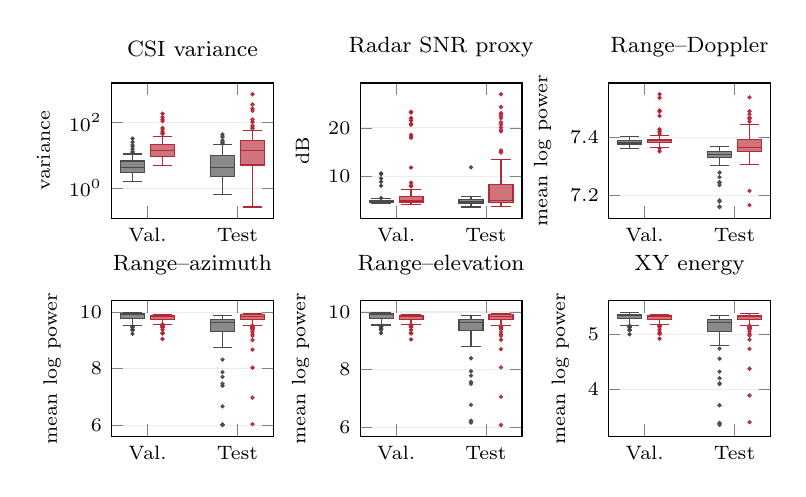
\begin{tikzpicture}
\begin{groupplot}[group style={group size=3 by 2,horizontal sep=1.1cm,vertical sep=1.05cm},width=.30\textwidth,height=3.3cm,boxplot/draw direction=y,xtick={1.5,4.5},xticklabels={Val.,Test},xmin=.3,xmax=5.7,tick label style={font=\scriptsize},title style={font=\footnotesize},label style={font=\scriptsize},ymajorgrids,grid style={gray!15}]
\nextgroupplot[title={CSI variance},ylabel={variance},ymode=log]
\addplot+[boxplot prepared={lower whisker=1.58073862,lower quartile=2.95647337,median=4.21875639,upper quartile=6.77691498,upper whisker=11.0541832},boxplot/draw position=1,fill=emptycolor!65,draw=emptycolor,mark=*,mark size=.55pt] coordinates {(1,32.5289368) (1,12.6773784) (1,20.9705334) (1,25.5212785) (1,15.6679949) (1,12.737123) (1,18.9847951)};
\addplot+[boxplot prepared={lower whisker=5.07282374,lower quartile=9.39278057,median=13.9613175,upper quartile=21.8681367,upper whisker=36.7124187},boxplot/draw position=2,fill=occColor!65,draw=occColor,mark=*,mark size=.55pt] coordinates {(2,47.7544301) (2,122.489002) (2,111.120852) (2,145.71773) (2,63.3416942) (2,44.9911888) (2,46.5537669) (2,68.7848917) (2,185.806582) (2,53.0986999)};
\addplot+[boxplot prepared={lower whisker=0.653086912,lower quartile=2.33979282,median=4.33478821,upper quartile=10.1151655,upper whisker=20.8638588},boxplot/draw position=4,fill=emptycolor!65,draw=emptycolor,mark=*,mark size=.55pt] coordinates {(4,22.7048666) (4,24.462451) (4,28.7754928) (4,43.6709869) (4,36.0947173) (4,27.1659135) (4,38.6452756)};
\addplot+[boxplot prepared={lower whisker=0.271108805,lower quartile=5.12254235,median=14.1373878,upper quartile=28.1121781,upper whisker=57.1782251},boxplot/draw position=5,fill=occColor!65,draw=occColor,mark=*,mark size=.55pt] coordinates {(5,104.034878) (5,67.0170331) (5,262.306641) (5,354.329587) (5,123.709556) (5,227.152153) (5,73.8456248) (5,80.3285784) (5,725.593275)};
\nextgroupplot[title={Radar SNR proxy},ylabel={dB}]
\addplot+[boxplot prepared={lower whisker=4.43293905,lower quartile=4.74308014,median=4.86605048,upper quartile=5.06731355,upper whisker=5.4889102},boxplot/draw position=1,fill=emptycolor!65,draw=emptycolor,mark=*,mark size=.55pt] coordinates {(1,10.5125475) (1,8.11972427) (1,8.93446064) (1,9.63316727) (1,10.6677923) (1,5.61834288)};
\addplot+[boxplot prepared={lower whisker=4.27525234,lower quartile=4.80111098,median=4.99900174,upper quartile=5.90193355,upper whisker=7.3130393},boxplot/draw position=2,fill=occColor!65,draw=occColor,mark=*,mark size=.55pt] coordinates {(2,8.75009727) (2,7.98784542) (2,8.23307514) (2,17.9620647) (2,21.8659973) (2,11.8529892) (2,22.0079803) (2,20.6137371) (2,23.2711601) (2,20.8244038) (2,18.5456696) (2,18.1079941) (2,23.1276302) (2,21.4516811)};
\addplot+[boxplot prepared={lower whisker=3.78085589,lower quartile=4.60178447,median=4.82958102,upper quartile=5.22692549,upper whisker=5.92855453},boxplot/draw position=4,fill=emptycolor!65,draw=emptycolor,mark=*,mark size=.55pt] coordinates {(4,11.8911657)};
\addplot+[boxplot prepared={lower whisker=3.81694436,lower quartile=4.73353708,median=5.11930466,upper quartile=8.3360076,upper whisker=13.5149622},boxplot/draw position=5,fill=occColor!65,draw=occColor,mark=*,mark size=.55pt] coordinates {(5,19.278141) (5,15.2286634) (5,20.688612) (5,15.3703117) (5,19.498312) (5,21.128027) (5,21.9850655) (5,22.9761429) (5,24.2614136) (5,14.9467506) (5,26.8776665) (5,20.067215) (5,22.4074726) (5,22.7542496)};
\nextgroupplot[title={Range--Doppler},ylabel={mean log power}]
\addplot+[boxplot prepared={lower whisker=7.36233902,lower quartile=7.37799239,median=7.38290143,upper quartile=7.39124084,upper whisker=7.40447998},boxplot/draw position=1,fill=emptycolor!65,draw=emptycolor,mark=*,mark size=.55pt] coordinates {};
\addplot+[boxplot prepared={lower whisker=7.36614275,lower quartile=7.38302529,median=7.38893294,upper quartile=7.39465272,upper whisker=7.40624142},boxplot/draw position=2,fill=occColor!65,draw=occColor,mark=*,mark size=.55pt] coordinates {(2,7.35287857) (2,7.36339903) (2,7.42011547) (2,7.42142582) (2,7.53770638) (2,7.49424934) (2,7.49030447) (2,7.47518873) (2,7.42869282) (2,7.42838144) (2,7.41273165) (2,7.5501771)};
\addplot+[boxplot prepared={lower whisker=7.30385542,lower quartile=7.330634,median=7.3432188,upper quartile=7.3518784,upper whisker=7.36923122},boxplot/draw position=4,fill=emptycolor!65,draw=emptycolor,mark=*,mark size=.55pt] coordinates {(4,7.23596191) (4,7.27952194) (4,7.16177177) (4,7.18321991) (4,7.24586773) (4,7.16037846) (4,7.24495268) (4,7.17901325) (4,7.26362467)};
\addplot+[boxplot prepared={lower whisker=7.30737448,lower quartile=7.3520062,median=7.36457825,upper quartile=7.39250278,upper whisker=7.44599724},boxplot/draw position=5,fill=occColor!65,draw=occColor,mark=*,mark size=.55pt] coordinates {(5,7.46881104) (5,7.45532894) (5,7.53925562) (5,7.4913373) (5,7.46546841) (5,7.16700077) (5,7.48040867) (5,7.2162447)};
\nextgroupplot[title={Range--azimuth},ylabel={mean log power}]
\addplot+[boxplot prepared={lower whisker=9.53309441,lower quartile=9.76028204,median=9.90883255,upper quartile=9.92986512,upper whisker=9.99449062},boxplot/draw position=1,fill=emptycolor!65,draw=emptycolor,mark=*,mark size=.55pt] coordinates {(1,9.47917938) (1,9.48371983) (1,9.48793602) (1,9.35236645) (1,9.46950436) (1,9.3712101) (1,9.22839642) (1,9.39594936) (1,9.47539806)};
\addplot+[boxplot prepared={lower whisker=9.57280731,lower quartile=9.74767351,median=9.84263134,upper quartile=9.86719441,upper whisker=9.90603065},boxplot/draw position=2,fill=occColor!65,draw=occColor,mark=*,mark size=.55pt] coordinates {(2,9.45770454) (2,9.25584602) (2,9.56166649) (2,9.04710007) (2,9.37625217) (2,9.24240971) (2,9.50610924) (2,9.50413799) (2,9.51563168) (2,9.256567) (2,9.50368404) (2,9.4583931)};
\addplot+[boxplot prepared={lower whisker=8.73778915,lower quartile=9.31505346,median=9.62822819,upper quartile=9.7343998,upper whisker=9.87242031},boxplot/draw position=4,fill=emptycolor!65,draw=emptycolor,mark=*,mark size=.55pt] coordinates {(4,7.39189768) (4,8.31869221) (4,6.00323725) (4,6.66277218) (4,7.87251282) (4,6.01496458) (4,7.46766615) (4,6.02010393) (4,7.70591688)};
\addplot+[boxplot prepared={lower whisker=9.53907394,lower quartile=9.74607515,median=9.85431337,upper quartile=9.90137124,upper whisker=9.94919395},boxplot/draw position=5,fill=occColor!65,draw=occColor,mark=*,mark size=.55pt] coordinates {(5,9.22031403) (5,9.50050735) (5,9.4163475) (5,9.0100708) (5,9.43898392) (5,9.45095539) (5,9.40078354) (5,9.50002766) (5,9.31161404) (5,6.03206062) (5,9.39945793) (5,9.5062809) (5,9.1583662) (5,8.02836895) (5,6.96922493) (5,8.67121983)};
\nextgroupplot[title={Range--elevation},ylabel={mean log power}]
\addplot+[boxplot prepared={lower whisker=9.54819489,lower quartile=9.7648654,median=9.91047478,upper quartile=9.93120027,upper whisker=9.99245453},boxplot/draw position=1,fill=emptycolor!65,draw=emptycolor,mark=*,mark size=.55pt] coordinates {(1,9.4883604) (1,9.4929781) (1,9.49887657) (1,9.37142181) (1,9.48558807) (1,9.40123272) (1,9.26869488) (1,9.42873287) (1,9.50257206)};
\addplot+[boxplot prepared={lower whisker=9.57892609,lower quartile=9.74780893,median=9.841012,upper quartile=9.86783075,upper whisker=9.90284061},boxplot/draw position=2,fill=occColor!65,draw=occColor,mark=*,mark size=.55pt] coordinates {(2,9.47673416) (2,9.26282692) (2,9.55889893) (2,9.04639626) (2,9.37115479) (2,9.25572395) (2,9.51720905) (2,9.51511478) (2,9.52459145) (2,9.27042389) (2,9.51402473) (2,9.46922207)};
\addplot+[boxplot prepared={lower whisker=8.8059721,lower quartile=9.34207153,median=9.64458418,upper quartile=9.74339437,upper whisker=9.87784386},boxplot/draw position=4,fill=emptycolor!65,draw=emptycolor,mark=*,mark size=.55pt] coordinates {(4,7.50387812) (4,8.39181042) (4,6.17524529) (4,6.77235794) (4,7.94101572) (4,6.15762711) (4,7.56885862) (4,6.2215662) (4,7.79091787)};
\addplot+[boxplot prepared={lower whisker=9.51997375,lower quartile=9.74752712,median=9.85511875,upper quartile=9.89970946,upper whisker=9.94681644},boxplot/draw position=5,fill=occColor!65,draw=occColor,mark=*,mark size=.55pt] coordinates {(5,9.22801495) (5,9.5023365) (5,9.41486835) (5,9.03621674) (5,9.44874477) (5,9.45731926) (5,9.42264271) (5,9.31662941) (5,6.07444382) (5,9.40532684) (5,9.51439667) (5,9.17102909) (5,8.07731724) (5,7.0498085) (5,8.70758915)};
\nextgroupplot[title={XY energy},ylabel={mean log power}]
\addplot+[boxplot prepared={lower whisker=5.16585064,lower quartile=5.27994621,median=5.34657192,upper quartile=5.36512268,upper whisker=5.39985704},boxplot/draw position=1,fill=emptycolor!65,draw=emptycolor,mark=*,mark size=.55pt] coordinates {(1,5.14207363) (1,5.1424551) (1,5.14220095) (1,5.07489204) (1,5.13425636) (1,5.07369089) (1,4.99848986) (1,5.08333254) (1,5.15144587) (1,5.12109041)};
\addplot+[boxplot prepared={lower whisker=5.18108034,lower quartile=5.27154386,median=5.32666373,upper quartile=5.33732522,upper whisker=5.36180878},boxplot/draw position=2,fill=occColor!65,draw=occColor,mark=*,mark size=.55pt] coordinates {(2,5.13674259) (2,5.03664494) (2,4.91902351) (2,5.08480167) (2,5.01061583) (2,5.14641857) (2,5.14481926) (2,5.14965534) (2,5.00586033) (2,5.15630484) (2,5.13456535)};
\addplot+[boxplot prepared={lower whisker=4.7970829,lower quartile=5.0537051,median=5.21029782,upper quartile=5.262941,upper whisker=5.33227777},boxplot/draw position=4,fill=emptycolor!65,draw=emptycolor,mark=*,mark size=.55pt] coordinates {(4,4.09374475) (4,4.55636358) (4,3.39092493) (4,3.71018648) (4,4.32138062) (4,3.37699723) (4,4.10888529) (4,3.35233426) (4,4.73838997) (4,4.20149422)};
\addplot+[boxplot prepared={lower whisker=5.16556644,lower quartile=5.27004135,median=5.32393956,upper quartile=5.34675837,upper whisker=5.37706947},boxplot/draw position=5,fill=occColor!65,draw=occColor,mark=*,mark size=.55pt] coordinates {(5,5.0040164) (5,5.14613104) (5,5.09575081) (5,4.90170383) (5,5.11653996) (5,5.12240887) (5,5.10213566) (5,5.15105438) (5,5.0518508) (5,3.40296388) (5,5.09504461) (5,5.14636326) (5,4.97530937) (5,4.37252188) (5,3.88811922) (5,4.73426294)};
\end{groupplot}
\end{tikzpicture}
\caption{Native LaTeX feature boxplots on the balanced validation (80/class) and test (96/class) cohorts. Gray: empty; red: occupied. Boxes show quartiles, the center line is the median, whiskers extend to observations within 1.5 IQR, and points are outliers. CSI uses a logarithmic axis. Each radar map panel displays its mean log-power descriptor; learning uses all five descriptors in~\eqref{eq:pool}.}
\label{fig:boxes}
\end{figure*}

\section{Results and Discussion}
\subsection{Matched-cohort comparison}
Thirteen input sets and two classifiers yield 26 candidates. BA is $\tfrac12[\mathrm{TN}/(\mathrm{TN}+\mathrm{FP})+\mathrm{TP}/(\mathrm{TP}+\mathrm{FN})]$. On balanced evaluation sets it equals ordinary accuracy. AUC measures ranking, not the performance of the frozen threshold. Table~\ref{tab:results} uses the validation-selected classifier within each input set.

\begin{table}[t]
\centering\caption{100 Hz CSI experiment. Classifier and threshold are selected on validation only. All rows share the same balanced cohorts.}
\label{tab:results}\footnotesize
\begin{tabular}{lcccc}\toprule
Inputs & Model & Val. BA & Test BA & Test AUC\\\midrule
\ResultRows
\bottomrule\end{tabular}
\end{table}

The overall selected model is \SelectedFeatures{} (\SelectedModel{}), with validation BA \ValBA\% and AUC \ValAUC. Its threshold is \SelectedThreshold. Test BA is \TestBA\% and AUC is \TestAUC, with TN=$\TestTN$, FP=$\TestFP$, FN=$\TestFN$, and TP=$\TestTP$. CSI+SNR gives \SnrFusionBA\% BA; CSI+SNR+RD gives \RdBA\% BA and \RdAUC{} AUC. RA fusion gives \RaBA\% BA and full fusion gives \AllBA\%. These are descriptive test comparisons, not a rule for selecting the best test configuration.

\begin{figure}[t]
\centering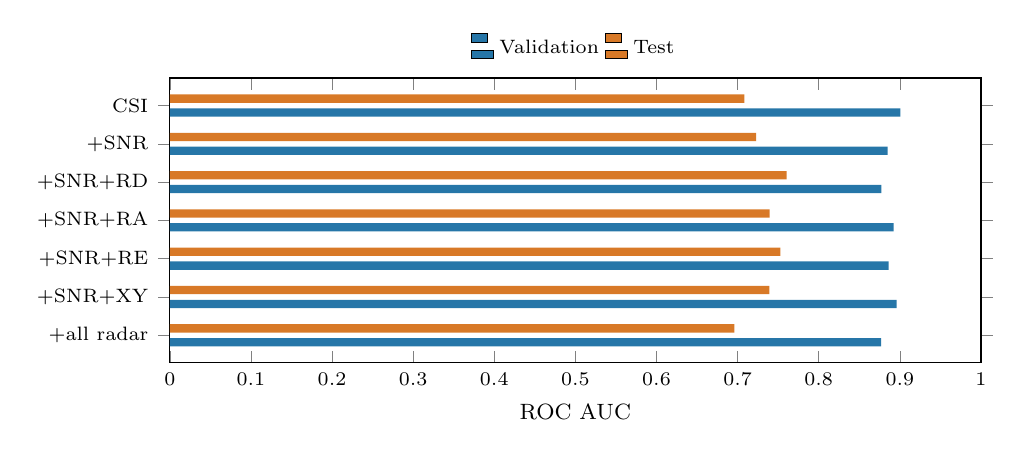
\begin{tikzpicture}
\begin{axis}[width=.98\columnwidth,height=5.2cm,xbar,bar width=3pt,xmin=0,xmax=1,ytick={0,1,2,3,4,5,6},yticklabels={CSI,{+SNR},{+SNR+RD},{+SNR+RA},{+SNR+RE},{+SNR+XY},{+all radar}},y dir=reverse,xlabel={ROC AUC},tick label style={font=\scriptsize},label style={font=\footnotesize},legend style={font=\scriptsize,at={(.5,1.03)},anchor=south,legend columns=2,draw=none},enlarge y limits=.12]
\addplot[fill=valColor,draw=none] coordinates {(0.90078125,0) (0.885,1) (0.87734375,2) (0.892421875,3) (0.886171875,4) (0.89609375,5) (0.87703125,6)};
\addplot[fill=testColor,draw=none] coordinates {(0.70844184,0) (0.722873264,1) (0.760416667,2) (0.739366319,3) (0.752604167,4) (0.739040799,5) (0.696126302,6)};
\legend{Validation,Test}
\end{axis}
\end{tikzpicture}
\caption{Validation and test ROC AUC for CSI and fusion variants. Classifiers are selected by validation balanced accuracy, with AUC breaking ties. AUC summarizes ranking across decision thresholds.}
\label{fig:performance}
\end{figure}

In a controlled preprocessing ablation on identical minute IDs, native-rate summaries give 67.2\% BA for CSI and 69.3\% for CSI+SNR+RD, compared with \CsiBA\% and \RdBA\% after resampling. Uniform sampling standardizes the processing grid, but does not improve these test operating points. The comparison retains the training observations, radar features, classifiers, and evaluation subsets; PCA and thresholds are refitted for each CSI representation.

\subsection{Coverage, transfer, and interpretation}
Every collected validation and test minute still contains the required features. This means at least one valid three-second CSI window and sufficient radar evidence, not uninterrupted measurements. Median accepted CSI support is \ValValidSeconds{} seconds per validation minute and \TestValidSeconds{} per test minute. Interpolation can smooth local variation; the source fingerprint, gap statistics, and interpolated counts are saved to make this effect inspectable.

The class boxes overlap and shift between sessions (Fig.~\ref{fig:boxes}). More descriptors do not imply more independent information: all radar views share one sensor, and XY derives from RA. Map pooling also discards spatial structure. The current experiment cannot isolate whether poor transfer arises from placement, hardware, background, label error, or their combination. It therefore does not establish that raw radar is uninformative.

\subsection{Computation and limitations}
The representation uses fixed PCA projection and conventional classifiers. LR inference scales linearly with feature count; a depth-4, 200-tree forest needs at most about 800 internal decision tests. These structural bounds are not a measured speed advantage. Radar decoding, FFTs, beamforming, and observation time may dominate. No matched deep-learning runtime or energy benchmark was performed.

Adjacent minutes and overlapping windows are dependent. Undersampling changes class prevalence without removing this dependence. The same evaluation sessions have been examined during development, including the decision to shorten CSI windows. Thus scores are exploratory, not a new untouched holdout. Sleep is absent from validation/test, and no three-class claim follows. A prospective session with verified geometry, stationary occupants, outside-view motion, and empty-room disturbances is required to confirm practical benefit.

\section{Conclusion}
We defined a complete mathematical path from WiFi observations $x_1$ and radar observations $x_2$ to compact branch features, fusion, and binary occupancy decisions. A guaranteed-rate routine supplies 100 Hz CSI before PCA; the resulting three-second variance preserves full minute-level feature availability on balanced evaluation cohorts. The validation-selected classifier reaches \TestBA\% test BA. Uniform sampling improves comparability of processing, but measured results do not establish an accuracy or speed advantage. The dataset manifests, source fingerprint, fixed split IDs, and native LaTeX figures support reproducible follow-up experiments.

\begin{thebibliography}{9}
\bibitem{wifi} G. Gad, I. Batool, M. Fouda, S. Verma, and Z. M. Fadlullah, ``WiFi Sensing-Based Human Activity Recognition for Smart Home Applications Using Commodity Access Points,'' supplied manuscript, 2026.
\bibitem{hood} S. M. Kahya, M. S. Yavuz, and E. Steinbach, ``HOOD: Real-Time Human Presence and Out-of-Distribution Detection Using FMCW Radar,'' arXiv:2308.02396, version 2, Mar. 2024. \url{https://arxiv.org/abs/2308.02396}.
\bibitem{deman} C. Wu et al., ``Non-Invasive Detection of Moving and Stationary Human With WiFi,'' \emph{IEEE J. Sel. Areas Commun.}, vol. 33, no. 11, pp. 2329--2342, 2015, doi: 10.1109/JSAC.2015.2430294.
\bibitem{sharp} F. Meneghello et al., ``SHARP: Environment and Person Independent Activity Recognition With Commodity IEEE 802.11 Access Points,'' \emph{IEEE Trans. Mobile Comput.}, 2023, doi: 10.1109/TMC.2022.3185681.
\bibitem{litehar} H. Salehinejad and S. Valaee, ``LiteHAR: Lightweight Human Activity Recognition from WiFi Signals with Random Convolution Kernels,'' in \emph{Proc. ICASSP}, 2022, doi: 10.1109/ICASSP43922.2022.9746803.
\bibitem{fusion} Z. Chen, Y. Sun, and L. Qu, ``Research on Cross-Scene Human Activity Recognition Based on Radar and Wi-Fi Multimodal Fusion,'' \emph{Electronics}, vol. 14, no. 8, art. 1518, 2025, doi: 10.3390/electronics14081518.
\end{thebibliography}
\end{document}
